%%%
% Some general discussion about the JH functions that we're gonna reference
% later.
%%%
The JH family of hash functions are a set of functions that were submitted to
the NIST SHA-3 competition. The submission defines four specific hash
algorithms: JH-224, JH-256, JH-384, and JH-512. All of these separate functions
are implemented through a very similar construction, and as such one would
expect them to exhibit similar performance properties as well as optimization
opportunities.

Wu\cite{wu2008jh} describes the hash function family in his submission to the
NIST competition. JH is constructed through a simple to describe compression
function that is shared by all variants. The compression function maintains
$1024$ bits of internal state and operates on $512$ bit blocks at a time. Even
before doing performance analysis, this would indicate that we should expect to
see a jump in the number of cycles required every $64$ bytes, as at those byte
boundaries the function has to process another block of data. The differences
between the functions are in how the context of the hash is seeded and how much
of the data is taken off the end to form the digest, and so we would expect to
see similar performance across all of the JH functions.

%%%
% The JH-224 Variant.
%%%
\subsubsection{JH-224}
\begin{figure}[H]
    \begin{center}
        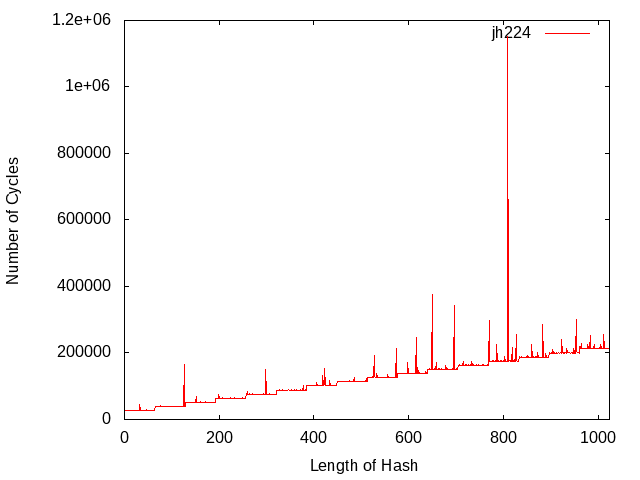
\includegraphics[scale=0.5]{images/jh224.png} 
        \caption{JH-224 with 224-bit output}
    \end{center}
\end{figure}

The algorithm selected for benchmarking JH-224 was bitslice\_opt32 compiled with
\texttt{gcc -mcpu=arm920t -O2 -fomit-frame-pointer} with GCC version 4.4.5. This
choice makes sense given the 32 bit word length of this Snapdragon processor,
and the fact that JH is designed such that bitslicing is an effective
optimization technique\cite{wu2008jh}. 

We note that the prediction that there would be a jump in the number of cycles
used every $64$ bytes was confirmed. We further note that each jump appears to
be roughly equivalent, implying that they are attributable to similar phenomena,
further confirming our suspicions. 

Wu\cite{wu2008jh} gives details about the bit-slicing implementation used for
JH. The implementation he defines performs bit-slicing optimizations on
components of the 512-bit block used in the encryption permutation, and leaves
the overall construction largely unaffected. This explains why we still see the
$64$ byte block boundaries playing an important roll in defining the shape of
the performance graph.


%%%
% The JH-256 Variant.
%%%
\subsubsection{JH-256}
\begin{figure}[H]
    \begin{center}
        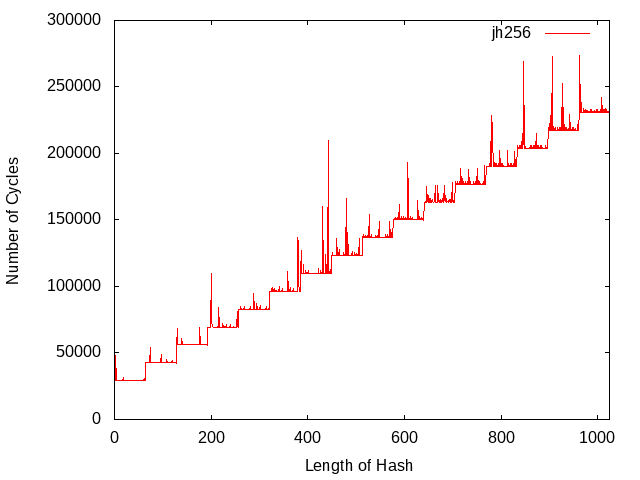
\includegraphics[scale=0.5]{images/jh256.png} 
        \caption{JH-256 with 256-bit output}
    \end{center}
\end{figure}

The algorithm selected for benchmarking JH-256 was bitslice\_opt32 compiled with
\texttt{gcc -mcpu=arm8 -O3 -fomit-frame-pointer} with GCC version 4.4.5. Again,
this choice of algorithm makes sense given that the Snapdragon processor has a
32 bit word length. Interestingly, different optimization options were selected
during the profiling process for JH-256 than for JH-224, however this would lead
us to believe that this implementation is designed in such a way that the
compiler is not given enough leeway to make meaningful optimizations based on
the differences.

We again note that our predicted graph shape held, and that the growth of this
function is roughly similar to that of JH-224. This is what we would expect
given that all variants of JH share a compression function.


%%%
% The JH-384 Variant.
%%%
\subsubsection{JH-384}
\begin{figure}[H]
    \begin{center}
        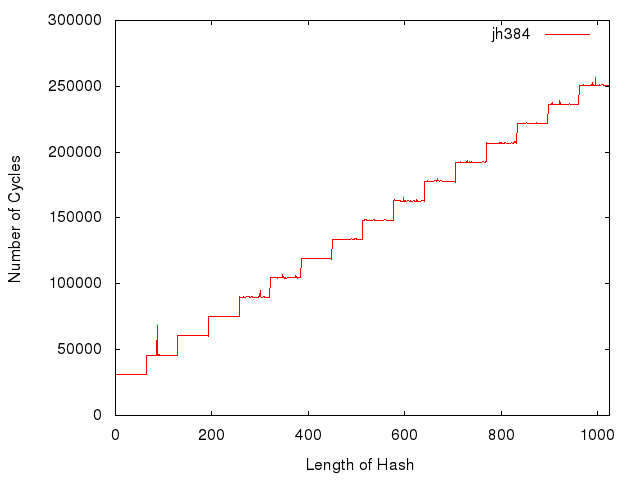
\includegraphics[scale=0.5]{images/jh384.png} 
        \caption{JH-384 with 384-bit output}
    \end{center}
\end{figure}

The algorithm selected for benchmarking JH-384 was bitslice\_ref32 compiled with
\texttt{gcc -mcpu=arm9 -O -fomit-frame-pointer} with GCC version 4.4.5.
Interestingly, this is a different algorithm from the other JH versions tested.
The selection of a $32$ bit reference implementation makes sense, given that the
Snapdragon processor has a $32$ bit word length. 

Although it is a different implementation, this implementation exhibits many of
the same qualities as the opt32 version. The stair step is exactly as we would
have predicted from an understanding of the algorithm, and the growth is roughly
on par with the other versions of JH. This would seem to imply that the
optimizations in the opt32 version are not much of an optimization over the
reference bit-sliced version for this board, and that bit-slicing is in and of
itself a very effective optimization.

%%%
% The JH-512 Variant.
%%%
\subsubsection{JH-512}
\begin{figure}[H]
    \begin{center}
        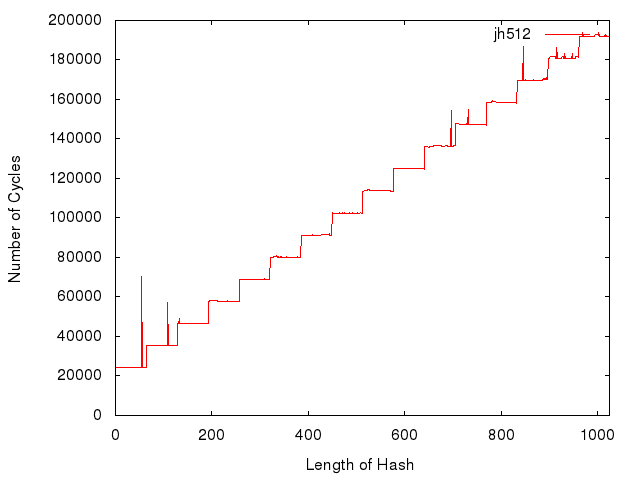
\includegraphics[scale=0.5]{images/jh512.png} 
        \caption{JH-512 with 512-bit output}
    \end{center}
\end{figure}

The algorithm selected for benchmarking JH-512 was bitslice\_opt32 compiled with
\texttt{gcc -mcpu=cortex-a9 -mfloat-abi=softfp -mfpu=neon -Os -fomit- \\
frame-pointer} with GCC version 4.4.5. This optimized algorithm makes sense for
the 32 bit Snapdragon processor, and given that JH is easily optimized through
bit-slicing. In this instance we have a different set of optimization
parameters, we do note a slight drop in the cycles consumed at the high levels
so perhaps optimization for the NEON FPU is beneficial or optimization for size
allows better management of the cache. Regardless, the performance graph is very
similar to the other graphs both in size and growth rate, and this can be
attributed to the shared compression function used across all lengths of JH.
